
\documentclass[runningheads]{llncs}
\usepackage{graphicx}
\usepackage{apacite}
\usepackage{float}
\usepackage{listings}
\lstset{
  basicstyle=\ttfamily,
  columns=fullflexible,
  frame=single,
  breaklines=true,
  postbreak=\mbox{\textcolor{red}{$\hookrightarrow$}\space},
}
\usepackage{float}
\usepackage[table]{xcolor}
\usepackage[toc,page]{appendix}
\usepackage{ucs}
\usepackage[utf8x]{inputenc}

\usepackage{hyperref}
\hypersetup{
	colorlinks=true,
	linkcolor=blue,
	filecolor=magenta,      
	urlcolor=cyan,
}

\usepackage[slovene]{babel}
\selectlanguage{slovene}

\lstset{
    breaklines=true,
    breakatwhitespace=true,
    inputencoding=utf8,
    extendedchars=false,
}

\renewcommand{\baselinestretch}{1.2} % za boljšo berljivost večji razmak
\renewcommand{\appendixpagename}{\normalfont\Large\bfseries{Appendix}}

\begin{document}

\title{Seminarska naloga}
\subtitle{Implementacija algoritma za grupiranje in določanja vodja grupe}

\author{Danijel Maraž, Nejc Rebernik}

\institute{Fakulteta za Računalništvo in Informatiko UL
\email{dm9929@student.uni-lj.si}\\
}

\maketitle             

\begin{abstract}
The article covers the work done in the scope of the seminar assignment as part of the subject wireless sensor networks.

\keywords{Raft nRF24LO1 Leader Consensus Wemos ESP}
\end{abstract}

\section{Uvod}
TODO tukaj povedat ključne cilje projekta 

\section{Splošna struktura}
splošen opis kode
\subsection{Election task}
opis taska, čemu služi itd. slikica
\subsection{Listen and react task}
opis delovanja taska slikica
\subsection{Device table}
kako deluje device table glej funkcije
\section{nRF24}
tukaj povedat kako poteka komunikacija s pomočjo modula:
bistvo je da se auto acknowledgement paketki ne avtomatsko pošiljajo in konstantno odpiramo pa zapiramo write in listen pipe da doseženo učinek broadcasta
\section{Raft}
opis rafta, vključi tudi robne primere ko vodja ni izvoljen ker ni dovolj glasov
\section{Protokol komunikacij}
\begin{figure}
  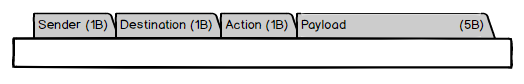
\includegraphics[width=\linewidth]{packet.png}
  \caption{Osnovna oblika paketa.}
  \label{fig:paket}
\end{figure}
slika paketka, v glavnem je maksimalen payload 8 bajtov na eno komunikacijo zato smo prve 3 rezervirali za naš addressing ostale pa za namišljen payload ki bi ga imeli v realni situaciji.
prvi bajt je zadnja črka MAC addressa ploščice, ki pošilja. drugi nam pove komu je pošiljka (F za broadcast) namenjena. tretji pa je funkcijski pomen, akcija E za election V za oddat glas A za acknowledge heartbeat H za heartbeat itd.
\section{One time pad}
opis one time pad. zakaj smo si ga izbrali (ker je simple). opis kako bi se dalo razbit vsebino komunikacij. imam samo en stalen ključ, ker bi bilo ponovno izmenjevanje preveč zapleteno gleda na nivo fleksibilnosti, ki ga imamo v našem sistemu wemosov.
\section{Primeri}
\begin{figure}
  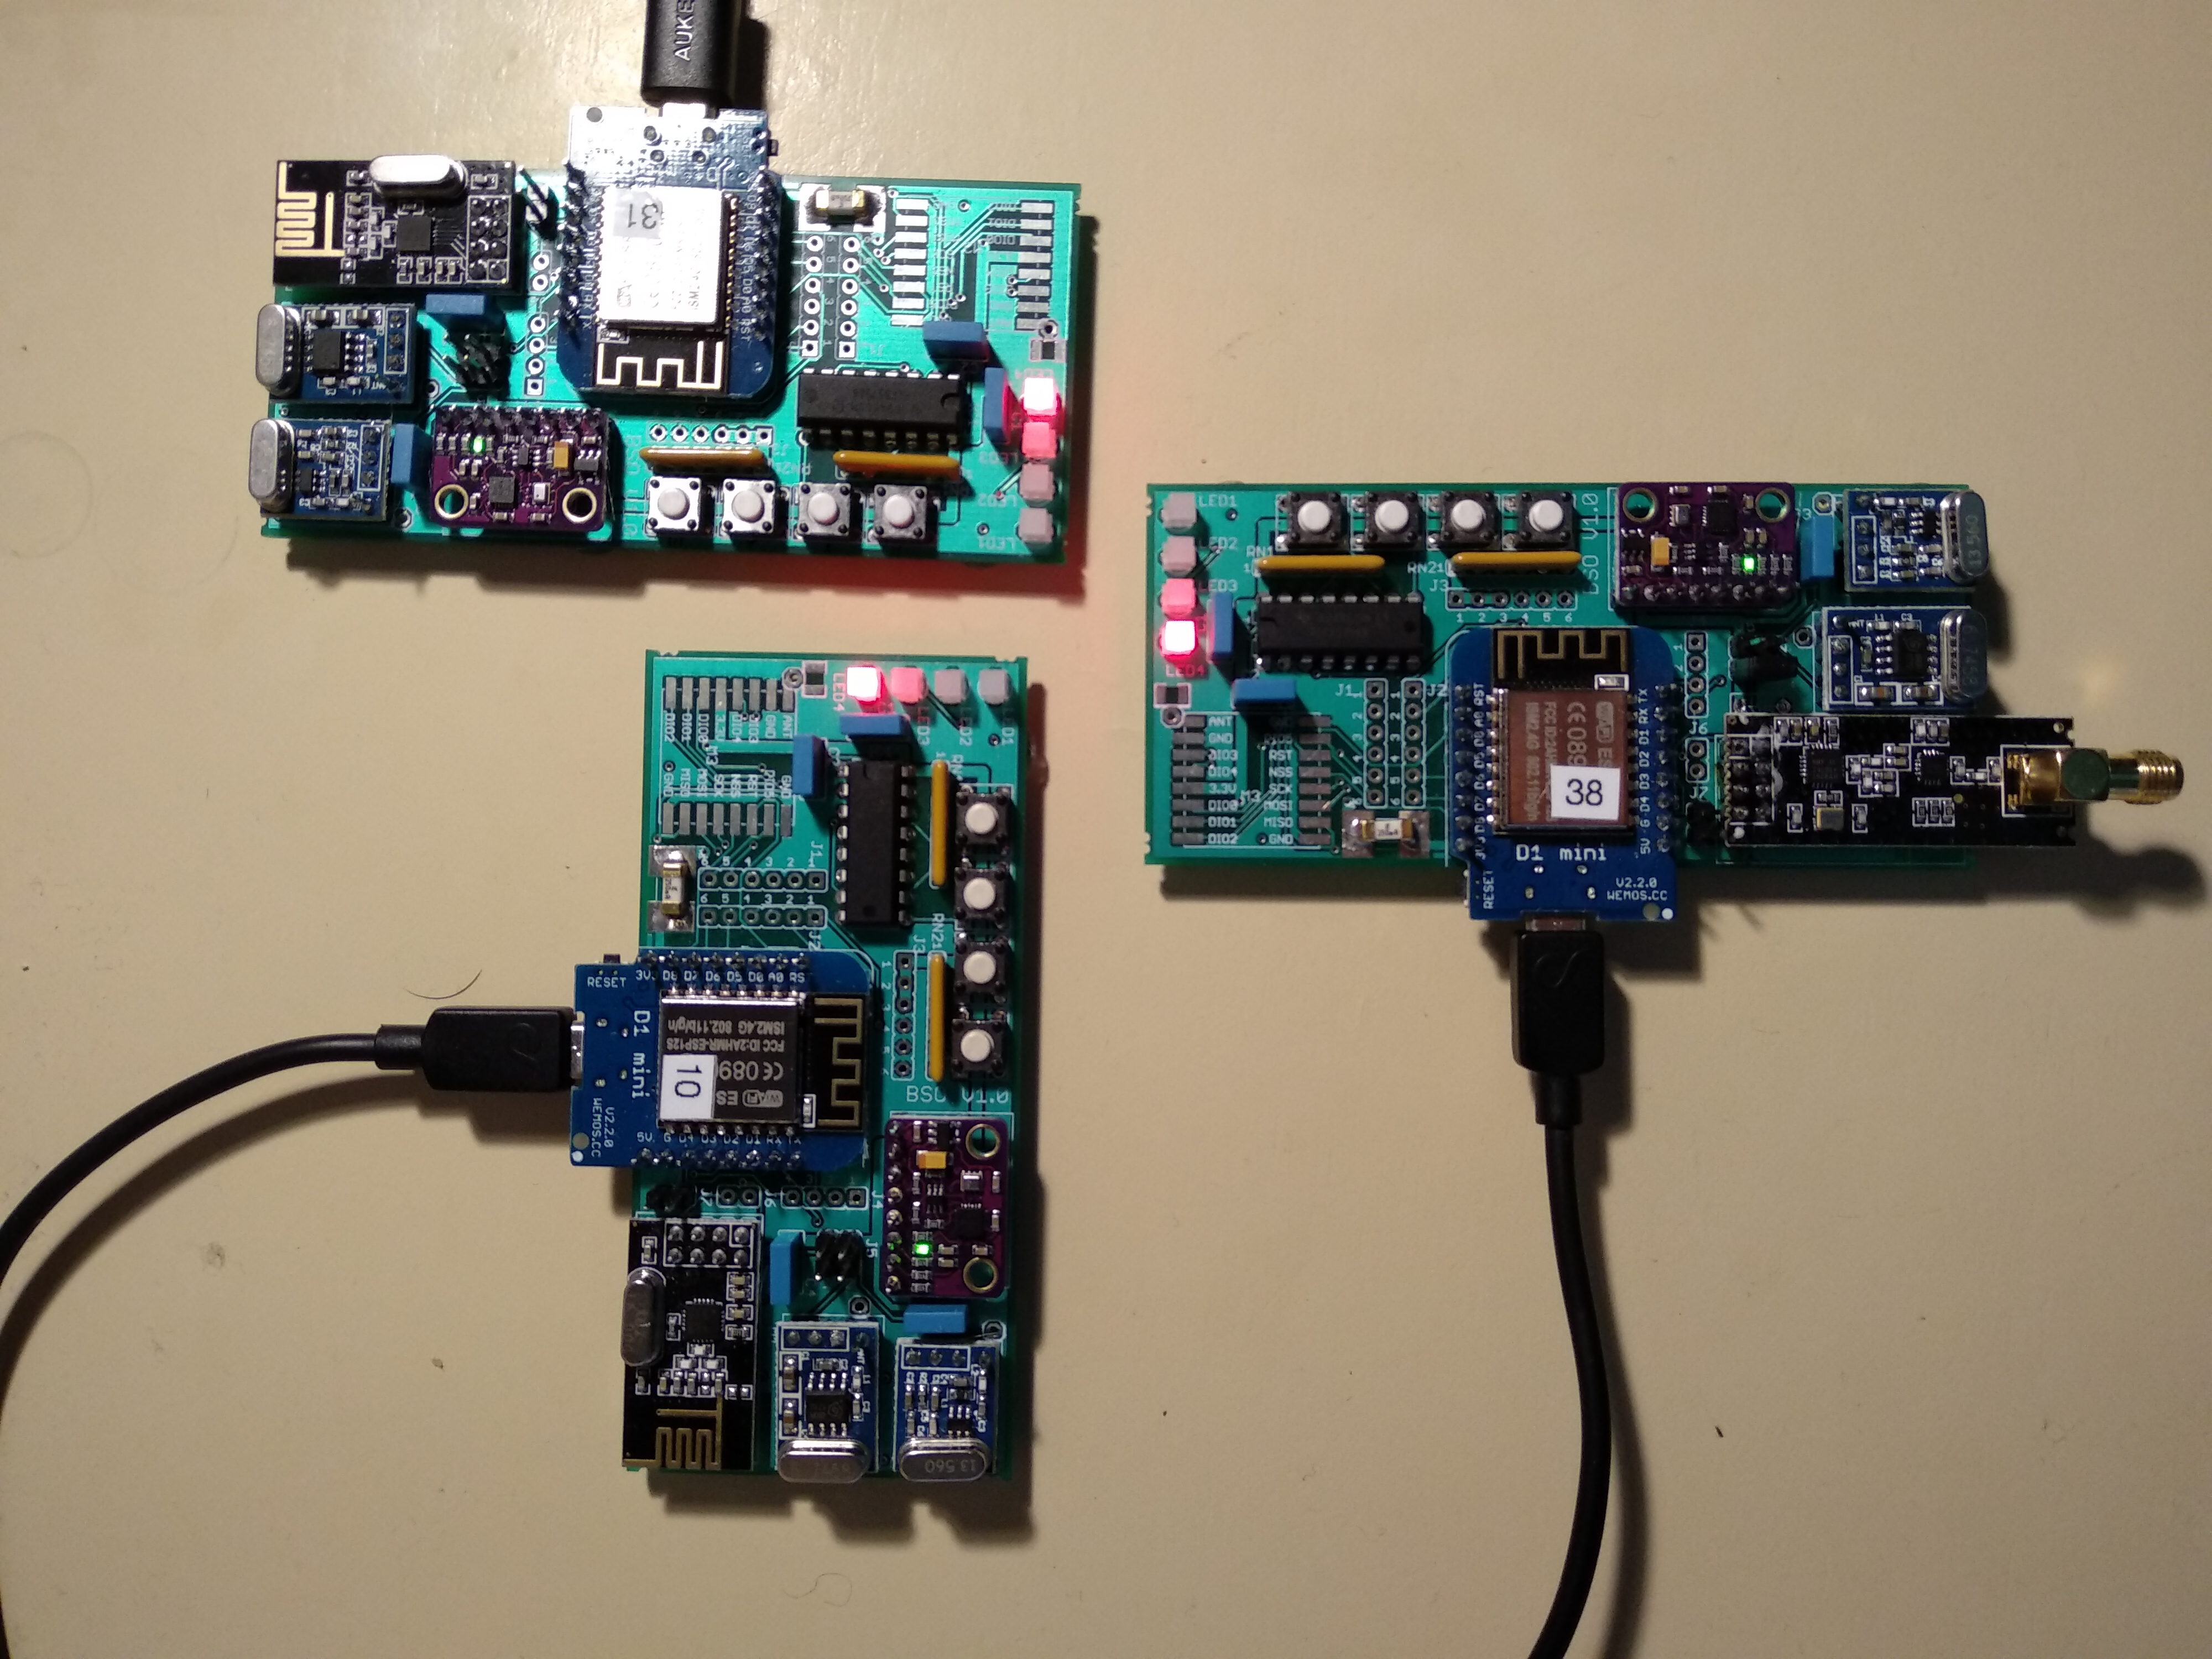
\includegraphics[width=\linewidth]{no_leader.jpg}
  \caption{Brez vodje bodo kmalu sledile nove volitve.}
  \label{fig:no_leader}
\end{figure}
\begin{figure}
  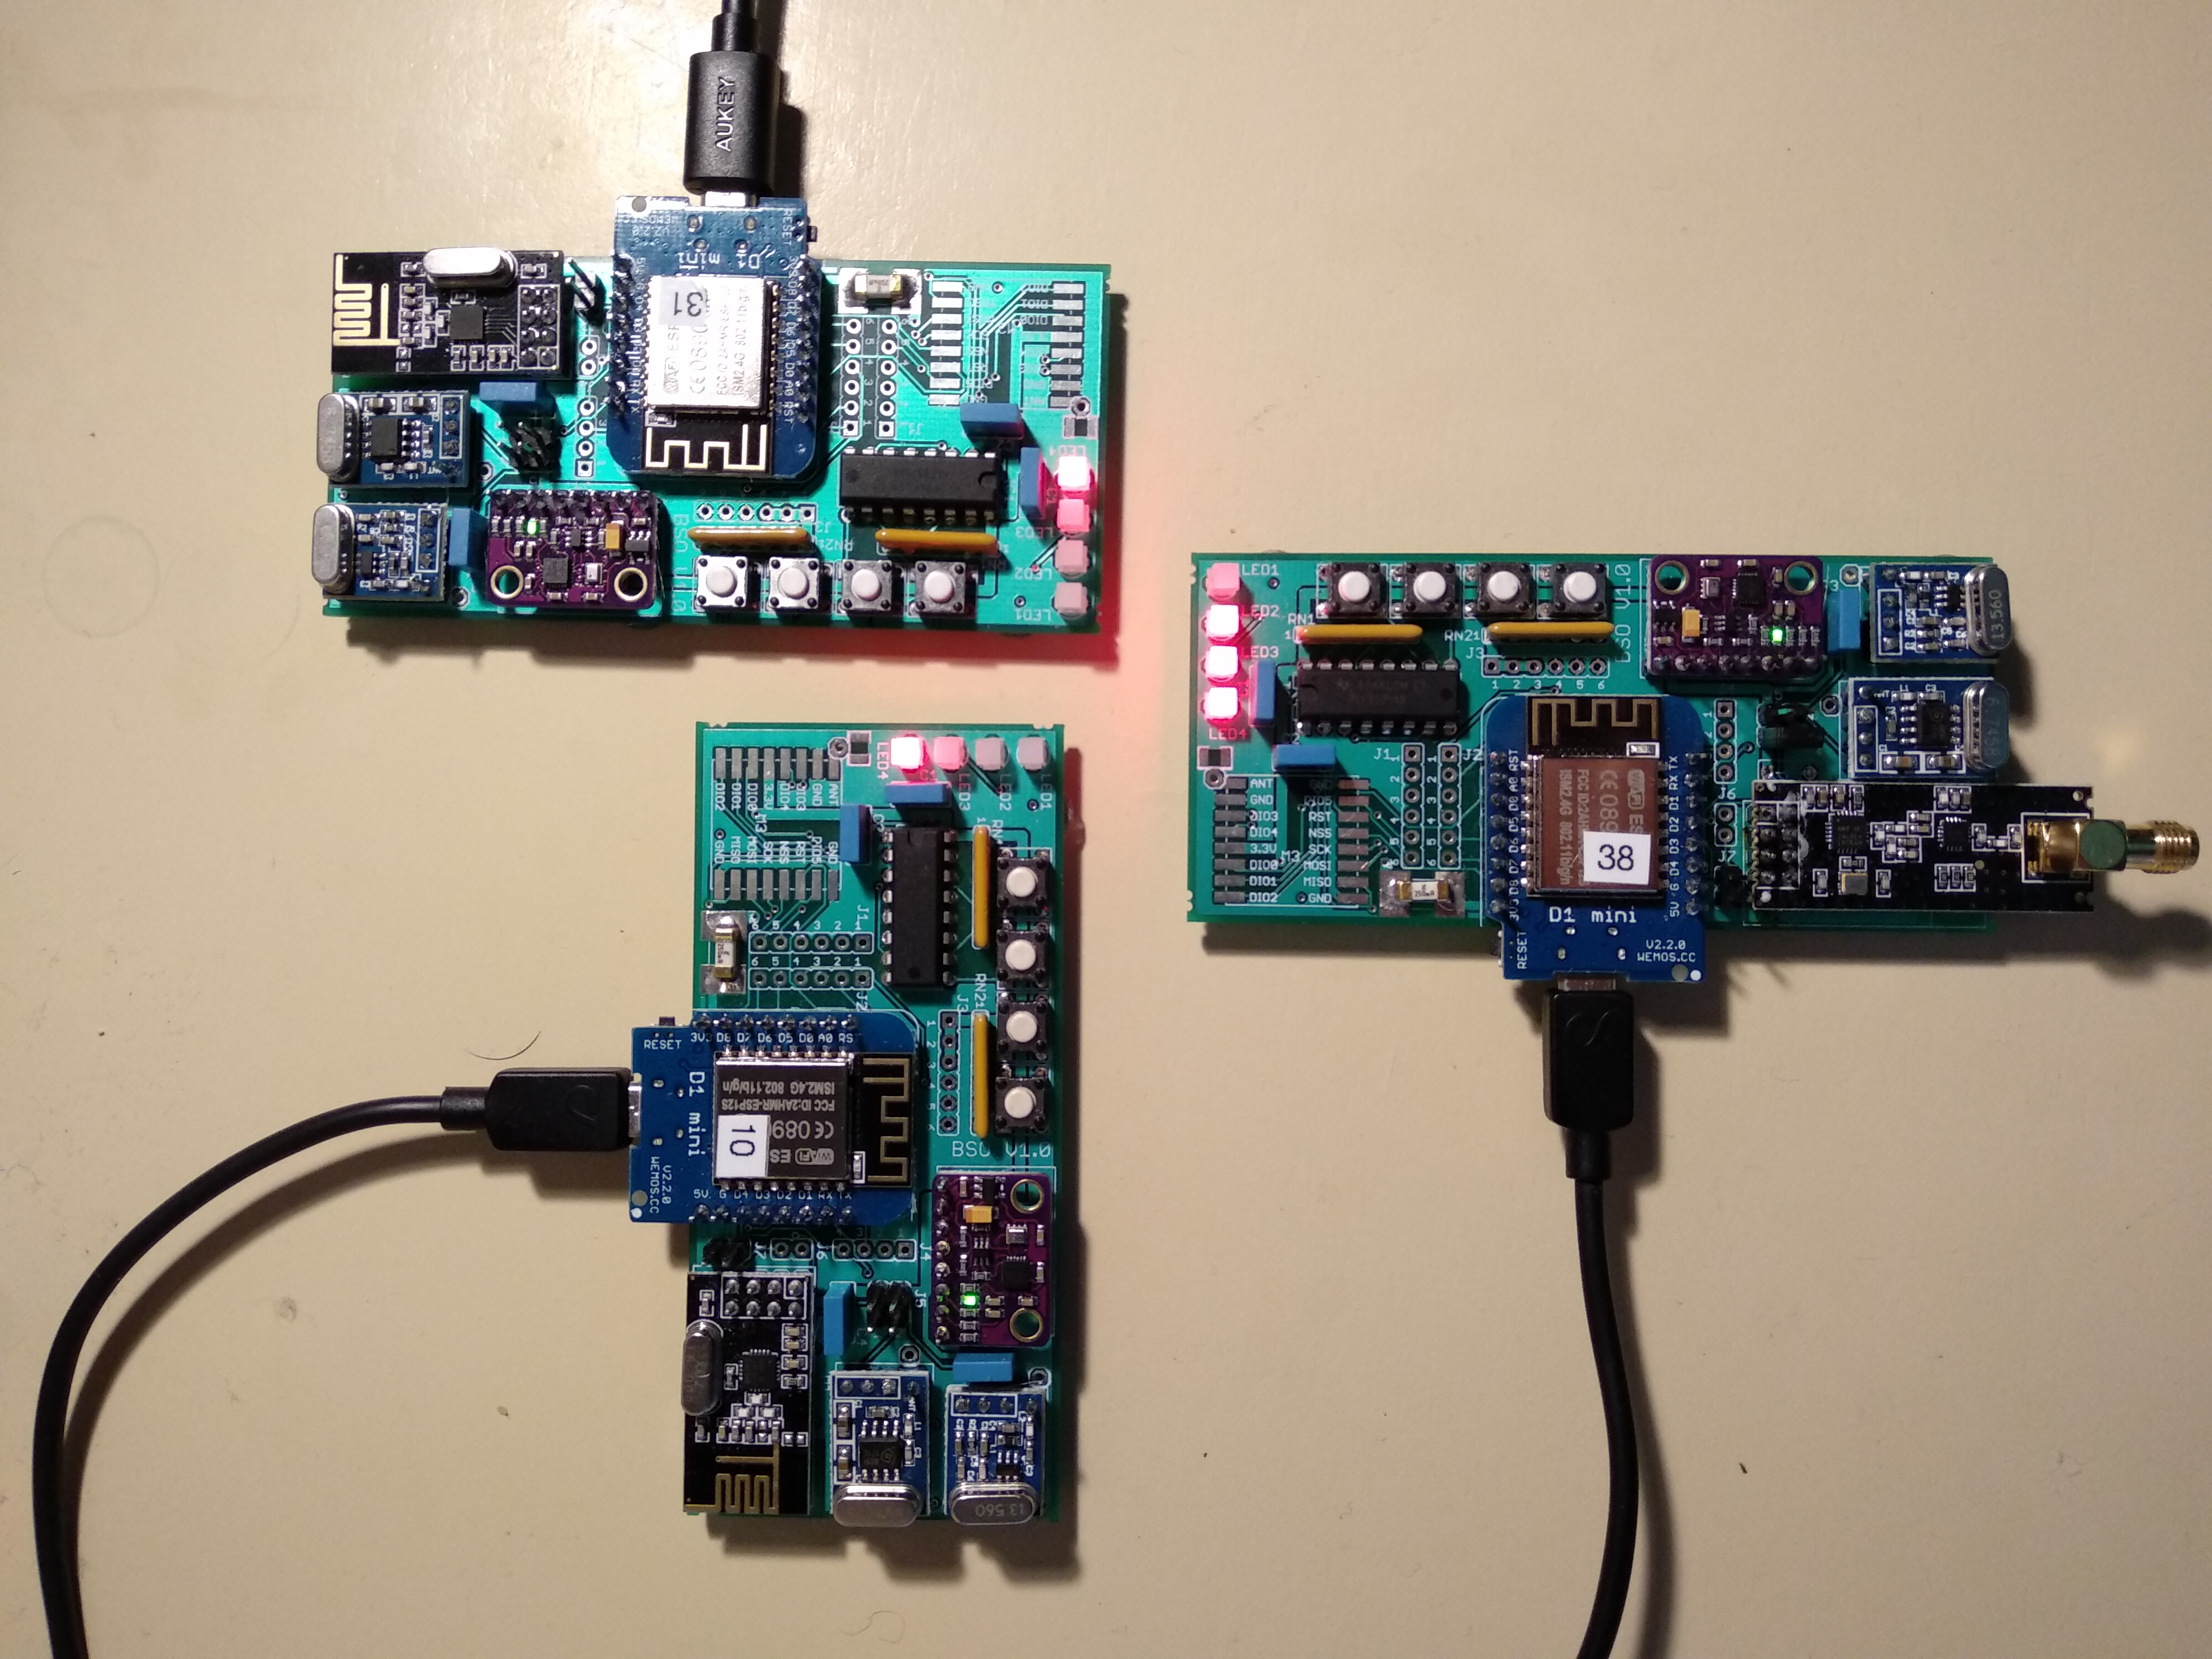
\includegraphics[width=\linewidth]{one_leader.jpg}
  \caption{Prisotnost vodje.}
  \label{fig:one_leader}
\end{figure}

\section{Zaključek}
dosežki projekta:
-delujoč določanje vodje (Raft)
-samo 1 preprosta koda za vsako napravo
-naprave se lahko poljubno priključijo v omrežje
-enkripcija one time pad
\end{document}

